% Chapter 2

\chapter{State of the Art: Agentic AI and Small Language Models in Healthcare} % Main chapter title

\label{chap:Chapter2} % For referencing the chapter elsewhere, use \ref{chap:Chapter2}

%----------------------------------------------------------------------------------------

\section{Research Methodology}

The systematic literature review was conducted following the PRISMA 2020 statement \cite{page2021prisma}, a framework designed to ensure transparency and reproducibility in systematic reviews. This methodology was selected for several compelling reasons that align with the nature of this research domain. First, the fields of Agentic AI, Small Language Models, and Vision-Language Models are characterized by rapid innovation cycles, with foundational architectures and benchmark results being superseded within months of publication. PRISMA's structured approach ensures that the evidence synthesis captures this dynamism while maintaining methodological rigor. Second, the framework's emphasis on explicit documentation of search strategies, inclusion criteria, and study selection processes enhances the reproducibility of findings---a critical consideration given the interdisciplinary nature of this work spanning computer science, medical informatics, and clinical dermatology.

The review process was structured into four distinct phases: (1) identification of relevant studies through systematic database searching; (2) screening of titles and abstracts based on predefined inclusion criteria; (3) eligibility assessment of full-text articles against methodological quality standards; and (4) qualitative synthesis of the selected studies to address the defined research questions. The temporal scope of the search spanned publications from January 2023 to January 2026, a period deliberately chosen to capture the rapid maturation of Small Language Models following the release of instruction-tuned models such as Llama-2, Mistral, and Phi-2. Studies published before 2023 were excluded from the systematic review but referenced as foundational works where necessary to establish theoretical context.

Quality assessment of the selected studies followed a structured appraisal protocol designed specifically for this research domain. Each study was evaluated against four criteria: (1) provision of direct quantitative comparisons between SLM-based systems and state-of-the-art LLMs; (2) explicit employment of multi-agent architectures or composite systems rather than single-model inference; (3) evaluation within specialized high-stakes domains requiring domain grounding; and (4) availability of reproducible artifacts such as open-source code, datasets, or detailed architectural specifications. This quality assessment framework ensures that the synthesized evidence directly addresses the research questions while maintaining standards appropriate for technical AI research.

\section{Research Questions}

The systematic review was guided by a hierarchical structure of research questions designed to comprehensively examine the viability of Small Language Models within agentic architectures for specialized domains. The Main Research Question (MRQ) establishes the central thesis under investigation, while the Sub-Research Questions (SRQs) decompose this inquiry into specific, addressable components that collectively inform the overarching question.

The Main Research Question driving this review is: 

\begin{center}
    \textbf{\textit{MRQ:} To what extent can Small Language Models achieve performance equivalence with Large Language Models in specialized domains through Agentic Architectures?}
\end{center}

This question emerges directly from the tension identified in Chapter~\ref{chap:Chapter1} between the demonstrated capabilities of massive foundation models and the practical constraints of computational cost, latency, and data privacy that limit their deployment in resource-constrained or privacy-sensitive contexts such as healthcare.
To systematically address this central question, four Sub-Research Questions were formulated, as presented in Table~\ref{tab:research_questions}.

\begin{table}[ht]
\centering
\caption{Sub-Research Questions and Their Rationale}
\label{tab:research_questions}
\renewcommand{\arraystretch}{1.4}
\begin{tabular}{|p{1.2cm}|p{6.5cm}|p{6.5cm}|}
\hline
\textbf{ID} & \textbf{Research Question} & \textbf{Rationale} \\
\hline
\textbf{SRQ1} & What are the limitations of Large Language Models that justify the architectural shift toward specialized Small Language Models? & Establishes the motivation for investigating alternatives to monolithic LLM architectures by examining their inherent constraints in deployment scenarios requiring efficiency, privacy, or specialized domain performance. \\
\hline
\textbf{SRQ2} & What are the key characteristics of Multi-Agent Systems compared to Monolithic Single-Agent architectures? & Understanding the architectural principles that enable distributed cognitive systems is essential for evaluating whether task decomposition and agent specialization can compensate for reduced model scale. \\
\hline
\textbf{SRQ3} & What is the comparative efficacy of Retrieval-Augmented Generation versus Parameter-Efficient Fine-Tuning for specializing Small Language Models? & Examines the two primary strategies for adapting smaller models to domain-specific tasks, informing the technical approach for the proposed system. \\
\hline
\textbf{SRQ4} & What evidence supports using fine-tuned Vision-Language Models over traditional computer vision approaches such as CNNs and ViTs? & Given the multimodal nature of dermatological diagnosis, this question investigates whether integrated vision-language architectures offer advantages over pipeline approaches. \\
\hline
\end{tabular}
\end{table}

\section{Search Strategy}

The search strategy was designed to ensure comprehensive coverage across the diverse publication venues characteristic of AI research while maintaining focus on the specific technical domains relevant to this dissertation. Given the rapid pace of development in generative AI, particular attention was paid to preprint repositories that often contain state-of-the-art results prior to formal peer review.

\subsection{Databases}

To capture relevant literature spanning computer science, medical informatics, and clinical research, the following databases and repositories were systematically searched:

\begin{table}[ht]
\centering
\caption{Databases Selected for Systematic Literature Search}
\label{tab:databases}
\begin{tabular}{p{0.22\textwidth}p{0.73\textwidth}}
\hline
\textbf{Database} & \textbf{Rationale for Inclusion} \\
\hline
\textbf{Google Scholar} &
Comprehensive coverage of academic literature across all disciplines, providing access to peer-reviewed papers, theses, books, and preprints. Serves as the primary discovery tool for cross-referencing findings across venues. \\
\hline
\textbf{arXiv} &
Open-access repository for electronic preprints in computer science, mathematics, and statistics. Given that state-of-the-art results in generative AI, language models, and multi-agent systems are frequently published here months before formal peer review, arXiv serves as the primary source for cutting-edge technical contributions. \\
\hline
\textbf{PubMed} &
The gold standard for biomedical literature, providing access to the MEDLINE database of peer-reviewed research in life sciences and clinical medicine. Essential for retrieving validated studies on dermatological diagnostics, telemedicine applications, and clinical AI evaluation methodologies. \\
\hline
\textbf{ACM Digital Library} &
Premier resource for computing and information technology research. Critical for accessing studies on multi-agent system architectures, efficient model deployment, and human-computer interaction in AI systems. \\
\hline
\textbf{Nature / Springer} &
High-impact peer-reviewed journals covering breakthrough research in medical AI, vision-language models, and clinical validation studies. Provides access to Nature Medicine, Nature Communications, and Scientific Reports publications. \\
\hline
\end{tabular}
\end{table}

\subsection{Search Terms}

The search strategy employed Boolean logic to combine keywords representing the four core pillars of this dissertation: (1) Health and Dermatology, (2) Generative AI, (3) Artificial Intelligence, and (4) System Architecture. Table~\ref{tab:search_terms} presents the search terms organized by domain category. The search strings were adapted to the syntax of each database while maintaining semantic equivalence across platforms.

\begin{table}[htbp]
\caption{Search Terms by Domain}
\label{tab:search_terms}
\renewcommand{\arraystretch}{1.3}
\begin{center}
\begin{tabular}{|l|p{10cm}|}
\hline
\textbf{Category} & \textbf{Search Terms} \\
\hline
Health & ``dermatology'' OR ``medical'' OR ``healthcare'' OR ``skin disease'' OR ``skin lesion'' OR ``skin cancer'' OR ``melanoma'' OR ``dermoscopy'' OR ``diagnosis'' OR ``clinical validation'' \\
\hline
Generative AI & ``large language model'' OR ``LLM'' OR ``small language model'' OR ``SLM'' OR ``Phi-3'' OR ``Gemma'' OR ``Llama'' OR ``Mistral'' OR ``retrieval augmented generation'' OR ``RAG'' OR ``knowledge distillation'' OR ``fine-tuning'' \\
\hline
Artificial Intelligence & ``vision language model'' OR ``VLM'' OR ``multimodal LLM'' OR ``CNN'' OR ``vision transformer'' OR ``LoRA'' OR ``PEFT'' OR ``quantization'' OR ``edge deployment'' OR ``privacy preserving'' \\
\hline
Architecture & ``multi-agent system'' OR ``MAS'' OR ``agentic AI'' OR ``task decomposition'' OR ``tool use'' OR ``orchestration'' OR ``benchmark'' OR ``evaluation'' OR ``hallucination mitigation'' \\
\hline
\end{tabular}
\end{center}
\end{table}

The search terms were combined using AND operators across domains to ensure retrieved studies addressed the intersection of AI methodology and healthcare application. For example, a typical combined query would be: (Health terms) AND (Generative AI terms) AND (Architecture terms).

\section{Selection Criteria}

The selection criteria were designed to identify studies that provide empirical evidence relevant to the research questions while ensuring methodological quality appropriate for informing system design decisions. The criteria balance inclusivity---necessary given the nascent state of SLM research---with rigor sufficient to support evidence-based conclusions.

\subsection{Inclusion Criteria}

Papers were included if they satisfied \textbf{all} of the following conditions:

\begin{enumerate}
    \item \textbf{Publication Date}: Published or made publicly available between January 2023 and January 2026, capturing the rapid evolution of instruction-tuned SLMs and their application in specialized domains.

    \item \textbf{Relevance to AI/ML Models}: The study must involve one or more of the following:
    \begin{itemize}
        \item Large Language Models (LLMs), Small Language Models (SLMs), Vision-Language Models (VLMs), or Multimodal Models
        \item Retrieval-Augmented Generation (RAG) techniques
        \item Multi-Agent or Agentic AI architectures
        \item Model optimization techniques (quantization, distillation, PEFT)
    \end{itemize}

    \item \textbf{Healthcare or Medical Domain}: Studies focusing on dermatology, skin disease classification, medical question-answering systems, or clinical decision support were prioritized to ensure direct relevance to the dissertation objectives.

    \item \textbf{Publication Type}: Peer-reviewed journal articles, conference papers from recognized venues (NeurIPS, ICML, ICLR, ACL, MICCAI), or high-quality preprints from established research groups (arXiv, medRxiv, bioRxiv) demonstrating methodological rigor.

    \item \textbf{Language}: Written in English.

    \item \textbf{Accessibility}: Full text available through institutional access or open access repositories.
\end{enumerate}

\subsection{Exclusion Criteria}

Papers were excluded if they met \textbf{any} of the following conditions:

\begin{enumerate}
    \item \textbf{Temporal Scope}: Published before January 2023, with the exception of seminal foundational works (e.g., the original Transformer architecture, LoRA) cited for background context but not included in the systematic synthesis.

    \item \textbf{Duplicate Publications}: Conference papers subsequently published as extended journal versions (journal version retained), or preprints superseded by peer-reviewed publications (peer-reviewed version retained).

    \item \textbf{Non-Generative AI Focus}: Studies on traditional machine learning approaches (SVMs, random forests, classical CNNs) without integration of language models or agentic components.

    \item \textbf{Non-Peer-Reviewed Sources}: Blog posts and technical documentation were excluded unless they represented official publications from major research organizations (e.g., NVIDIA, Microsoft Research, Google DeepMind).

    \item \textbf{Methodological Quality}: Studies without quantitative evaluation or lacking reproducibility details, as assessed through the quality appraisal framework.
\end{enumerate}

\subsection{Selection Process}

The selection process followed the PRISMA 2020 flow, progressing through identification, screening, eligibility assessment, and final inclusion. Figure~\ref{fig:prisma_diagram} illustrates the flow of studies through each phase of the review, documenting the number of records identified, screened, assessed for eligibility, and ultimately included in the qualitative synthesis.

\begin{figure}[H]
    \centering
    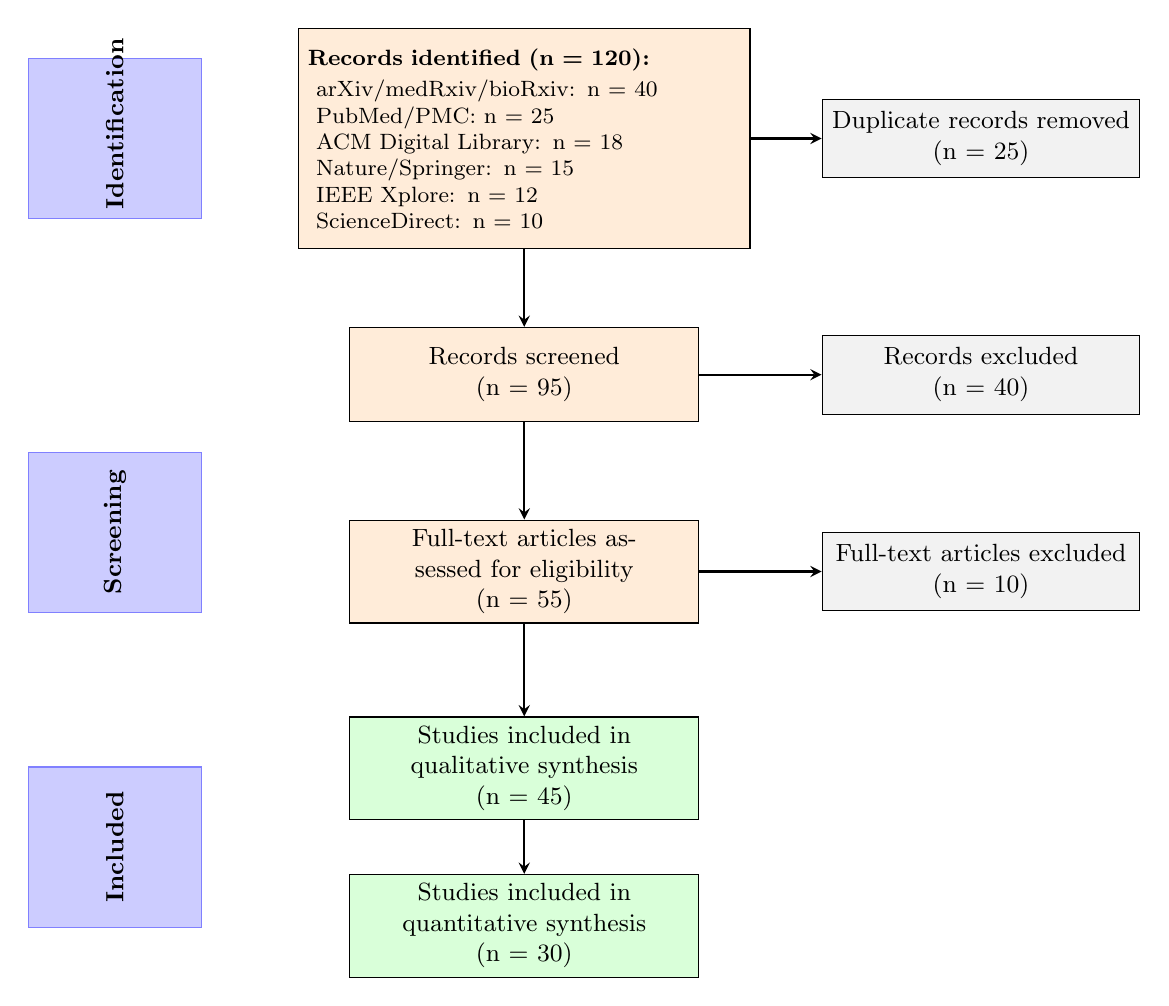
\begin{tikzpicture}[
        node distance=0.8cm and 1.2cm,
        box/.style={rectangle, draw=black, text width=4.2cm, minimum height=1.2cm, align=center, font=\small},
        dbbox/.style={rectangle, draw=black, text width=5.5cm, minimum height=2.8cm, align=left, font=\footnotesize},
        sidebox/.style={rectangle, draw=black, text width=3.8cm, minimum height=1cm, align=center, font=\small},
        phasebox/.style={rectangle, fill=blue!20, draw=blue!50, text width=1.8cm, minimum height=2.2cm, align=center, font=\small\bfseries, rotate=90},
        arrow/.style={->, >=stealth, thick}
    ]

    % Phase labels
    \node[phasebox] (id-label) at (-5.2, 0.5) {Identification};
    \node[phasebox] (sc-label) at (-5.2, -4.5) {Screening};
    \node[phasebox] (inc-label) at (-5.2, -8.5) {Included};

    % Identification phase - Database breakdown
    \node[dbbox, fill=orange!15] (identified) at (0, 0.5) {
        \textbf{Records identified (n = 120):}\\[2pt]
        \hspace{3pt}arXiv/medRxiv/bioRxiv: n = 40\\
        \hspace{3pt}PubMed/PMC: n = 25\\
        \hspace{3pt}ACM Digital Library: n = 18\\
        \hspace{3pt}Nature/Springer: n = 15\\
        \hspace{3pt}IEEE Xplore: n = 12\\
        \hspace{3pt}ScienceDirect: n = 10
    };
    \node[sidebox, fill=gray!10] (duplicates) at (5.8, 0.5) {Duplicate records removed\\(n = 25)};

    % Screening phase
    \node[box, fill=orange!15] (screened) at (0, -2.5) {Records screened\\(n = 95)};
    \node[sidebox, fill=gray!10] (excluded1) at (5.8, -2.5) {Records excluded\\(n = 40)};

    \node[box, fill=orange!15] (fulltext) at (0, -5) {Full-text articles assessed for eligibility\\(n = 55)};
    \node[sidebox, fill=gray!10] (excluded2) at (5.8, -5) {Full-text articles excluded\\(n = 10)};

    % Included phase
    \node[box, fill=green!15] (qualitative) at (0, -7.5) {Studies included in qualitative synthesis\\(n = 45)};
    \node[box, fill=green!15] (quantitative) at (0, -9.5) {Studies included in quantitative synthesis\\(n = 30)};

    % Arrows
    \draw[arrow] (identified.east) -- (duplicates.west);
    \draw[arrow] (identified.south) -- (screened.north);
    \draw[arrow] (screened.east) -- (excluded1.west);
    \draw[arrow] (screened.south) -- (fulltext.north);
    \draw[arrow] (fulltext.east) -- (excluded2.west);
    \draw[arrow] (fulltext.south) -- (qualitative.north);
    \draw[arrow] (qualitative.south) -- (quantitative.north);

    \end{tikzpicture}
    \caption{PRISMA 2020 flow diagram illustrating the systematic selection process. Records were identified from six academic databases, with arXiv and preprint servers contributing the largest share of AI/ML literature, followed by PubMed for medical domain coverage.}
    \label{fig:prisma_diagram}
\end{figure}

The initial database search identified approximately 120 records across the searched databases. After removing duplicates, 95 unique records underwent title and abstract screening against the inclusion criteria. Approximately 40 records were excluded at this stage, primarily due to insufficient relevance to generative AI architectures or lack of healthcare domain focus. The remaining 55 full-text articles were assessed for eligibility, with 10 excluded due to methodological limitations or redundancy with higher-quality studies addressing the same research questions. The final synthesis included 64 studies providing evidence relevant to one or more research questions, distributed across 12 thematic categories: SLMs as Future of Agentic AI (4 papers), Fine-tuned SLMs Outperforming LLMs (7 papers), Multi-Agent Systems (6 papers), Medical AI and Dermatology (10 papers), Knowledge Distillation (5 papers), RAG with SLMs (4 papers), Vision-Language Models (6 papers), Edge Deployment and Privacy (4 papers), Parameter-Efficient Fine-Tuning (5 papers), Model Quantization (4 papers), Hallucination Mitigation (4 papers), and Benchmarks (5 papers).

